\section{Classifiers Results and Discussion}

In this section, we present and analyze the results of the best candidate models obtained from both the traditional and \ac{dl} approaches.

The top-performing model from the traditional approach is an \ac{xgb} classifier, utilizing 33 audio features as input. This model achieved an accuracy of 60.69\% after performing 5-fold cross-validation on the \ac{iemo} dataset.

On the other hand, the final model obtained from the \ac{dl} approach is a Resnet50 model, which uses Spectrogram images as input. This model achieved an accuracy of 58.24\% using the same evaluation strategy and dataset.

Table \ref{final_models} shows the performance of final models that were trained using the entire \ac{iemo} dataset and then tested on three different datasets, namely eNTERFACE'05, EMO-DB, and CREMA-D.

The traditional model achieved the highest accuracy on the CREMA-D dataset with 48.88\%, followed by the eNTERFACE'05 dataset with 46.03\%, and the EMO-DB dataset with 38.94\%. On the other hand, the \ac{dl} model achieved the highest precision on the eNTERFACE'05 dataset with 52.13\%, followed by the CREMA-D dataset with 34.91\%, and the EMO-DB dataset with 12.78\%. However, the traditional model outperformed the \ac{dl} model on all other metrics, including macro F1, recall, and \ac{mcc}.

In terms of computation time, the traditional models were faster than the \ac{dl} models, which is evident from the lower time values in the table. This is a crucial factor when employing these models for real-time emotion recognition systems.

Moreover, in figure \ref{fig:final_cm} it is possible to observe that the models output "angry" several times indicating that it has difficulty distinguishing anger and happiness on these datasets. It was also noted from the EMO-DB confusion matrix, that the language of the data used is a limitation of the models' capacity, as this dataset's audio files are spoken in German. This highlights the English language bias of our \ac{ser} models and suggests that the results for other spoken languages may not be satisfactory.

Overall, these results indicate that the \ac{dl} model might be more effective for the \ac{ser} task on different datasets, due to its effective feature extraction and generalization capabilities. However, it is slower than the traditional models which can have a big impact when applied to real-time systems. We also recommend using these models for English audios, reducing the potential error caused by the language bias, since the results on a German dataset, EMO-DB, and on a dataset with varied accents, eNTERFACE'05 the results are not as good. It is also essential to acknowledge that \ac{dl} can yield even better results with more extensive models' hyperparameter tuning, which demands more computation time and power for their development and evaluation.


\begin{table}[H]
	\centering
	\caption{Final models trained on \ac{iemo} and evaluated on different datasets.}
	\label{final_models}
	\resizebox{\textwidth}{!}{%
		\rowcolors{2}{gray!25}{white}
		\begin{tabular}{llrrrrrr}
			\toprule
			Dataset & Model & Accuracy & Macro F1 & Precision & Recall & \ac{mcc} & Time \\
			\midrule
			\addlinespace[1mm]
			
			eNTERFACE'05 & Traditional & 29.37 & 18.61 & 17.85 & 22.02 & 0.064 & 0.18 \\
			& \acl{dl} & 36.67 & 22.91 & 44.36 & 27.50 & 0.087 & 0.25 \\
			
			\midrulec
			\addlinespace[1mm]
			
			EMO-DB & Traditional & 38.94 & 17.36 & 25.75 & 26.72 & 0.087 & 0.11 \\
			& \acl{dl} & 38.35 & 15.79 & 37.78 & 25.99 & 0.066 & 0.18 \\ 
			
			\midrulec
			\addlinespace[1mm]
			
			CREMA-D & Traditional & 44.41 & 35.45 & 63.18 & 46.12 & 0.335 &  0.11 \\
			& \acl{dl} & 54.14 & 47.71 & 51.68 & 52.98 & 0.407 & 0.30 \\
			
			\bottomrulec
		\end{tabular}%
	}
\end{table}


\begin{figure}
	\begin{subfigure}{.5\textwidth}
		\centering
		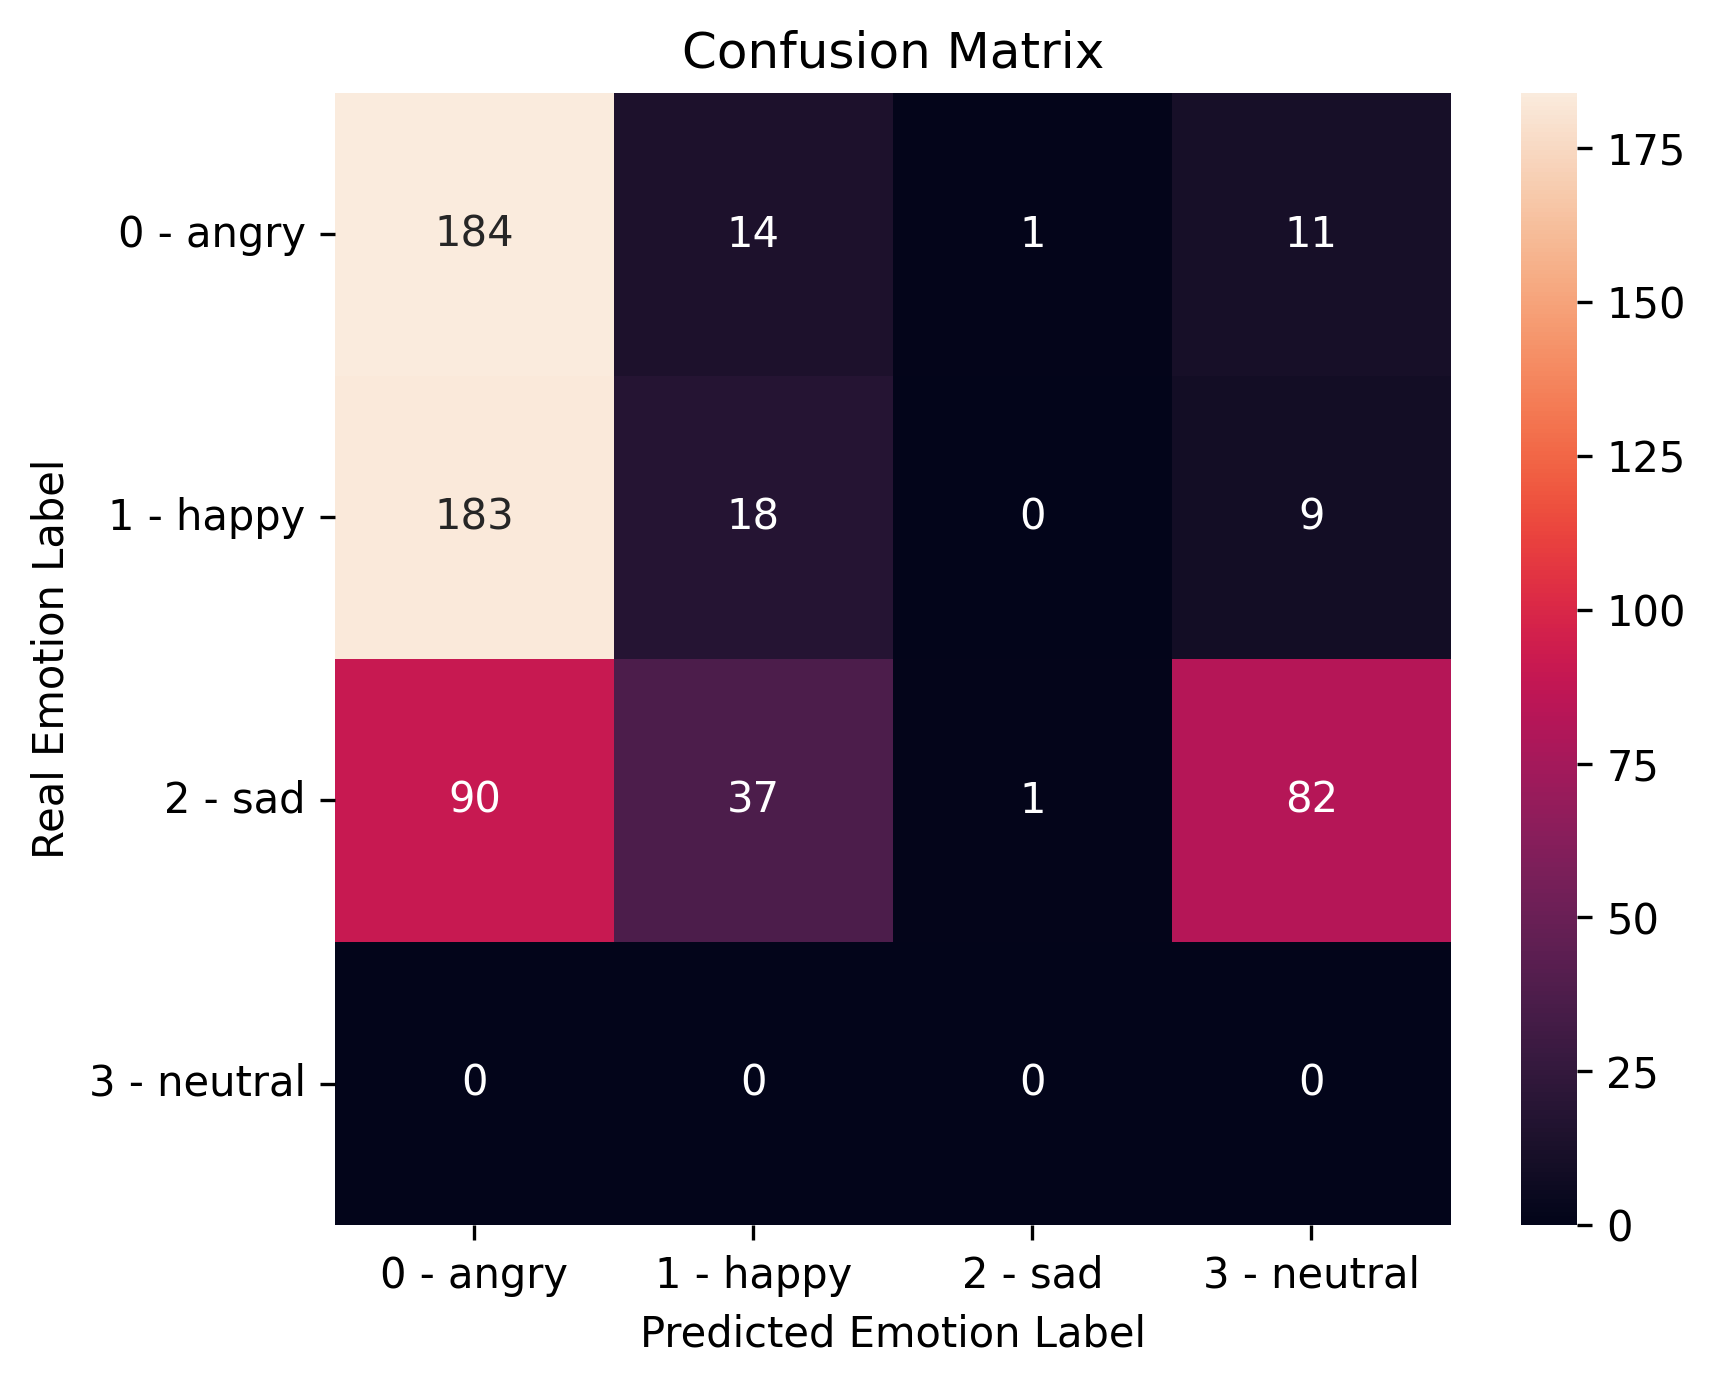
\includegraphics[width=\linewidth]{figs/4_5_discussion/ent_trad_cm.png}
		\caption{eNTERFACE'05 traditional model confusion matrix.}
	\end{subfigure}%
	\begin{subfigure}{.5\textwidth}
		\centering
		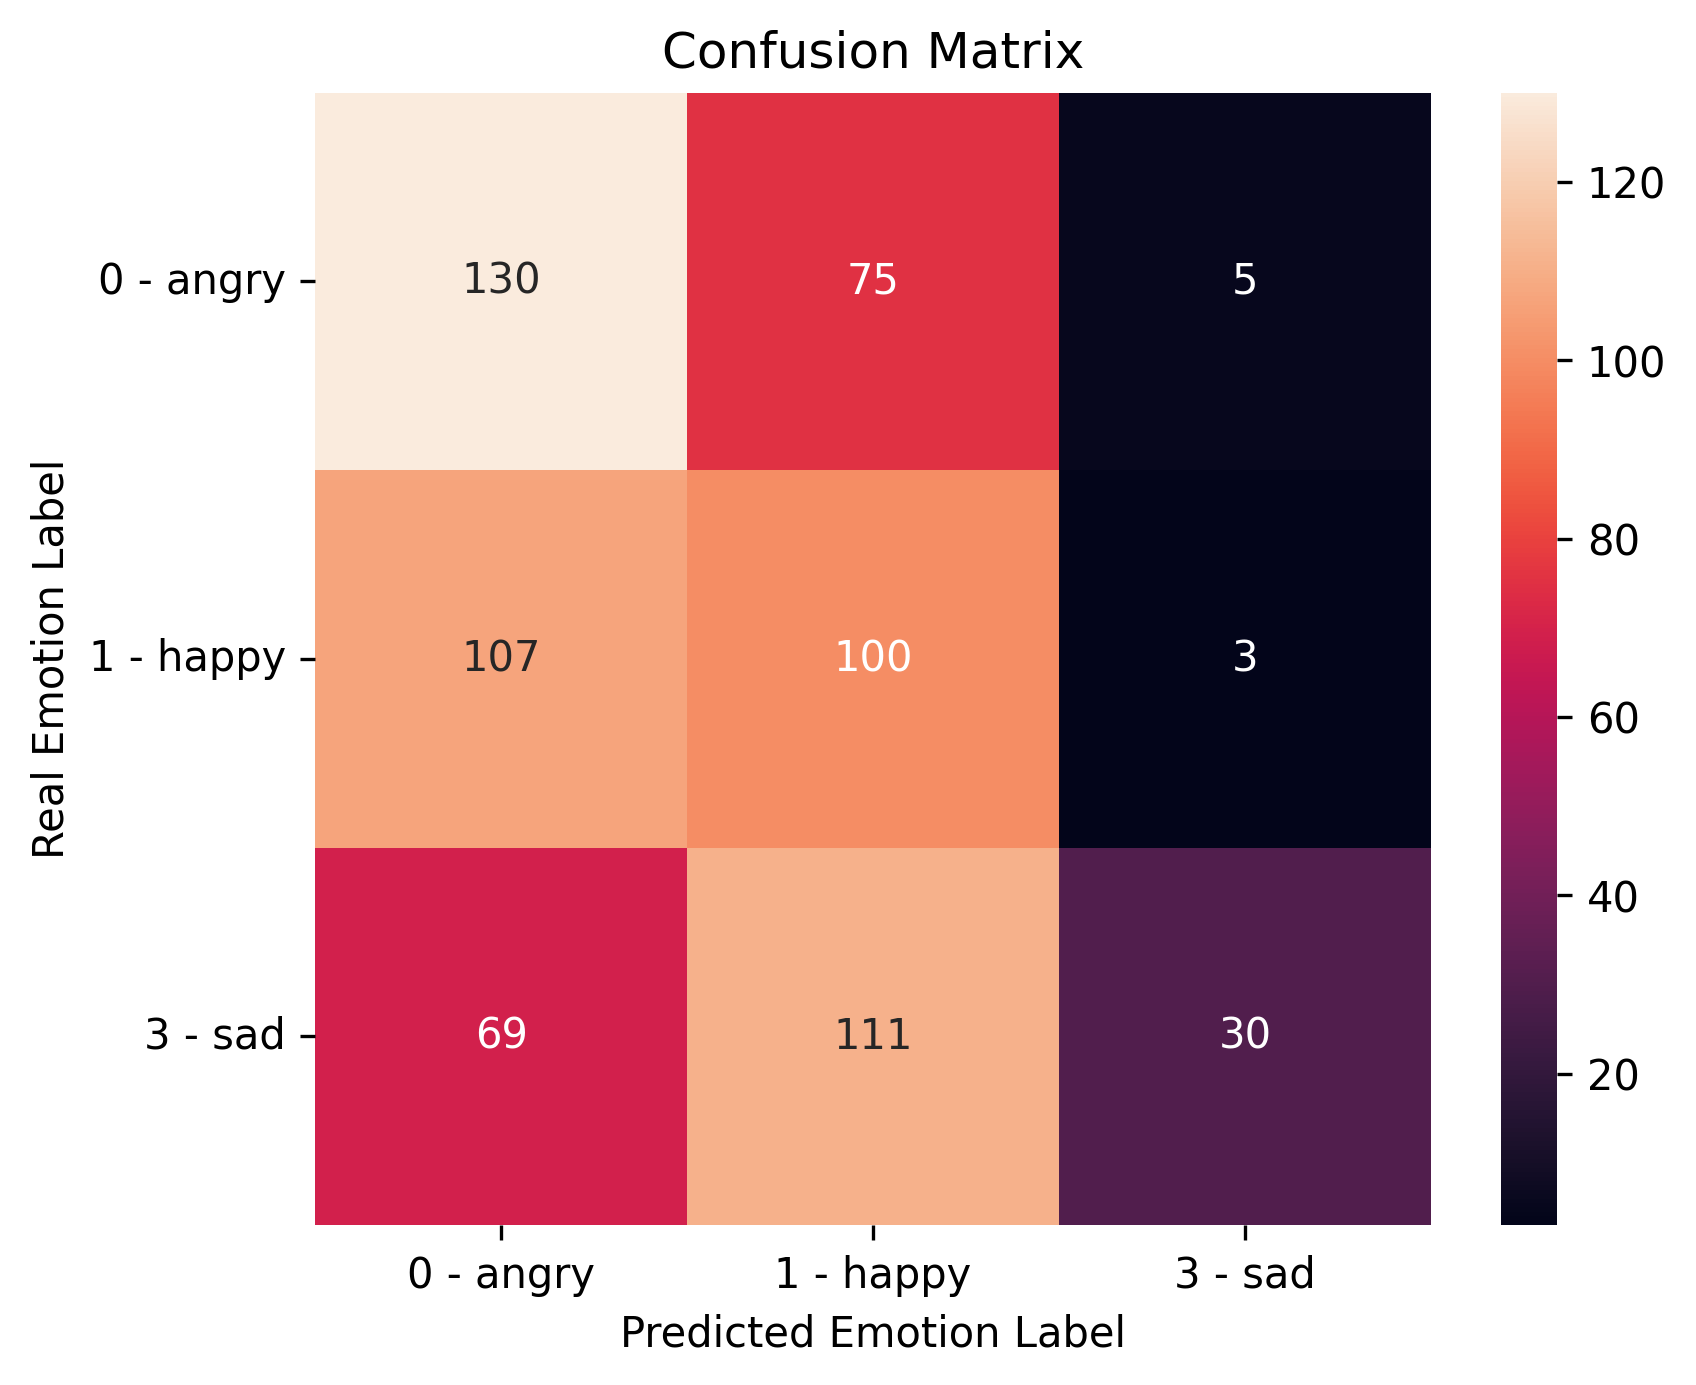
\includegraphics[width=\linewidth]{figs/4_5_discussion/ent_deep_cm.png}
		\caption{eNTERFACE'05 \ac{dl} model confusion matrix.}
	\end{subfigure}
	\newline
	\begin{subfigure}{.5\textwidth}
		\centering
		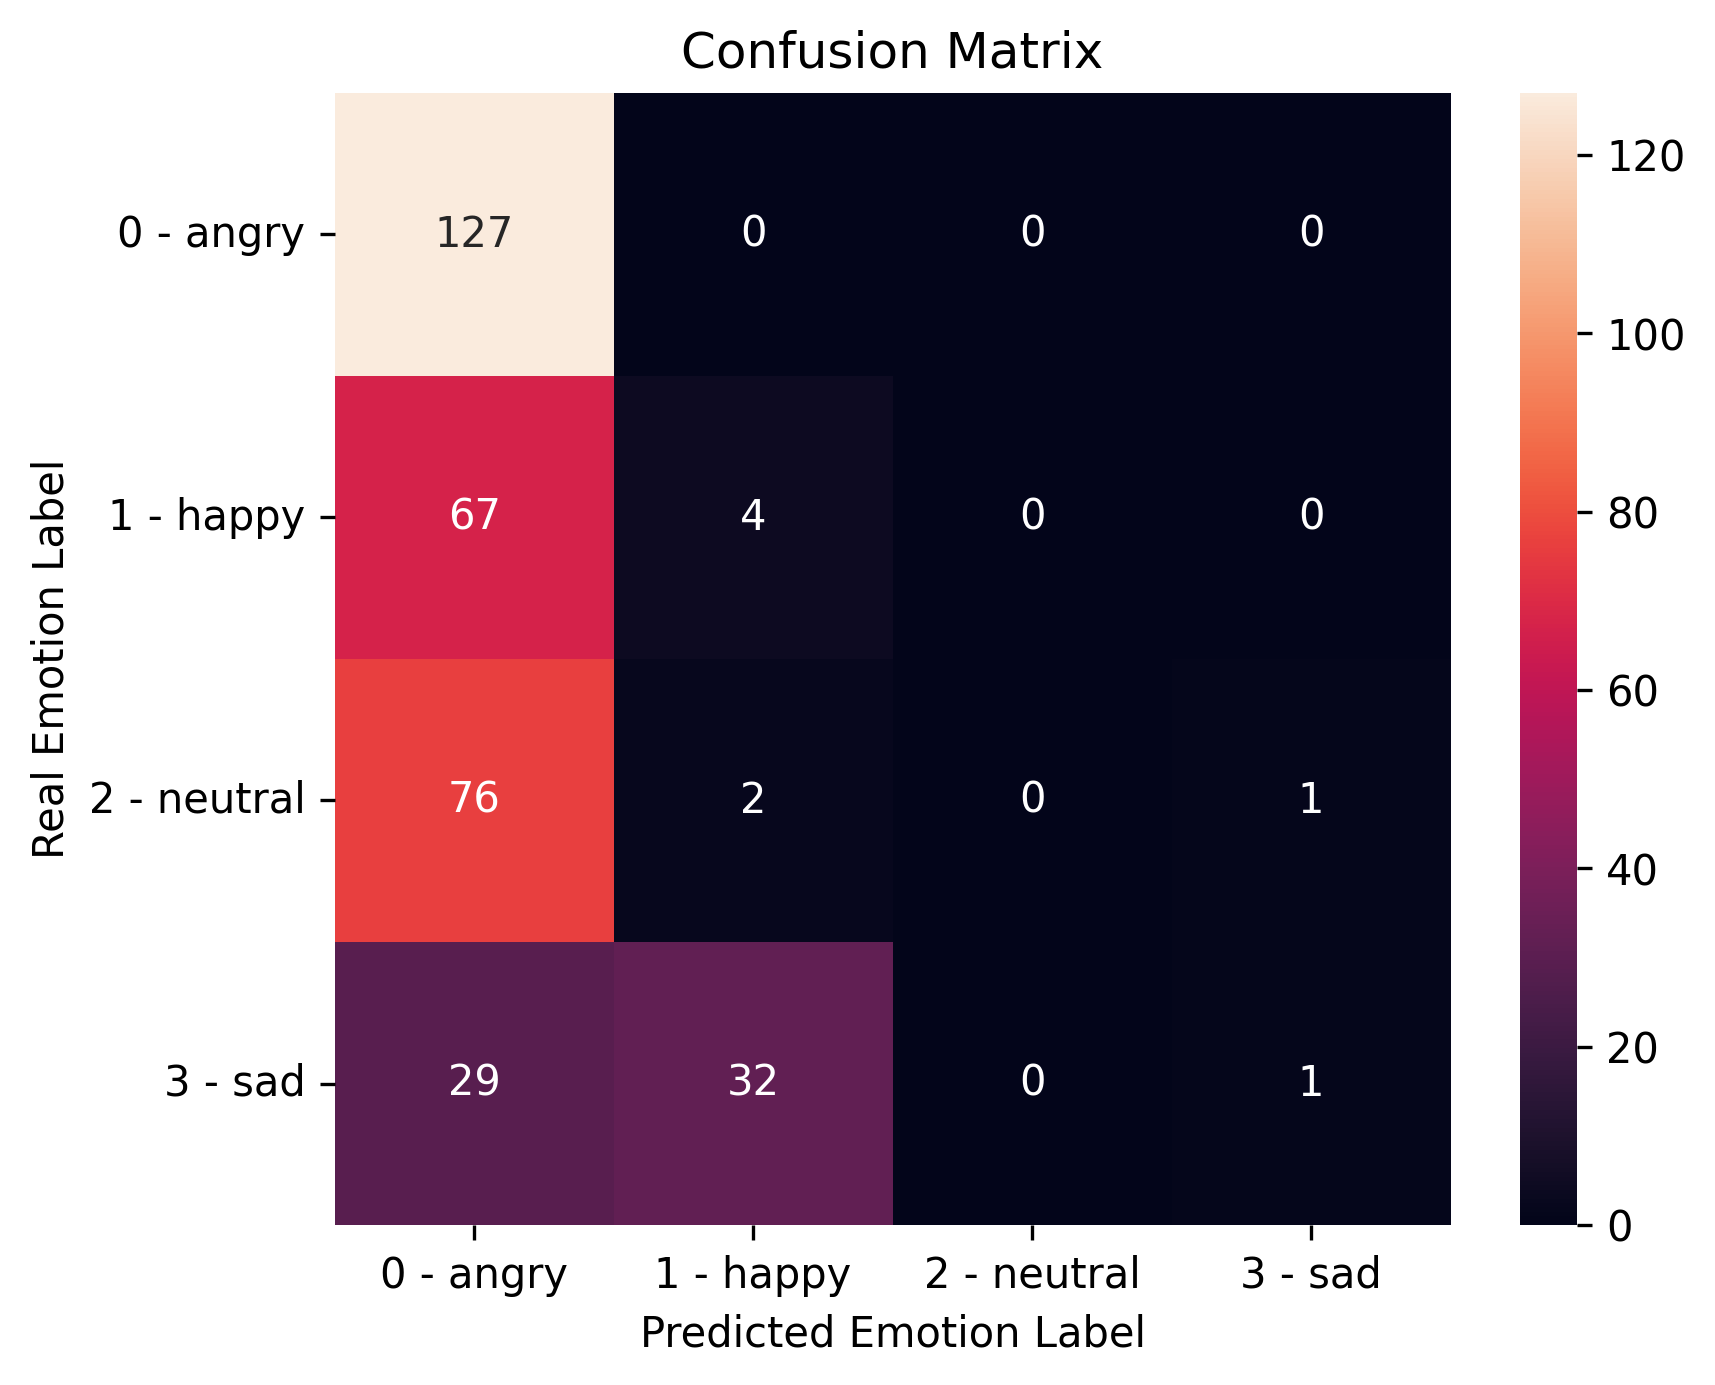
\includegraphics[width=\linewidth]{figs/4_5_discussion/emo_trad_cm.png}
		\caption{EMO-DB Traditional model confusion matrix.}
	\end{subfigure}%
	\begin{subfigure}{.5\textwidth}
		\centering
		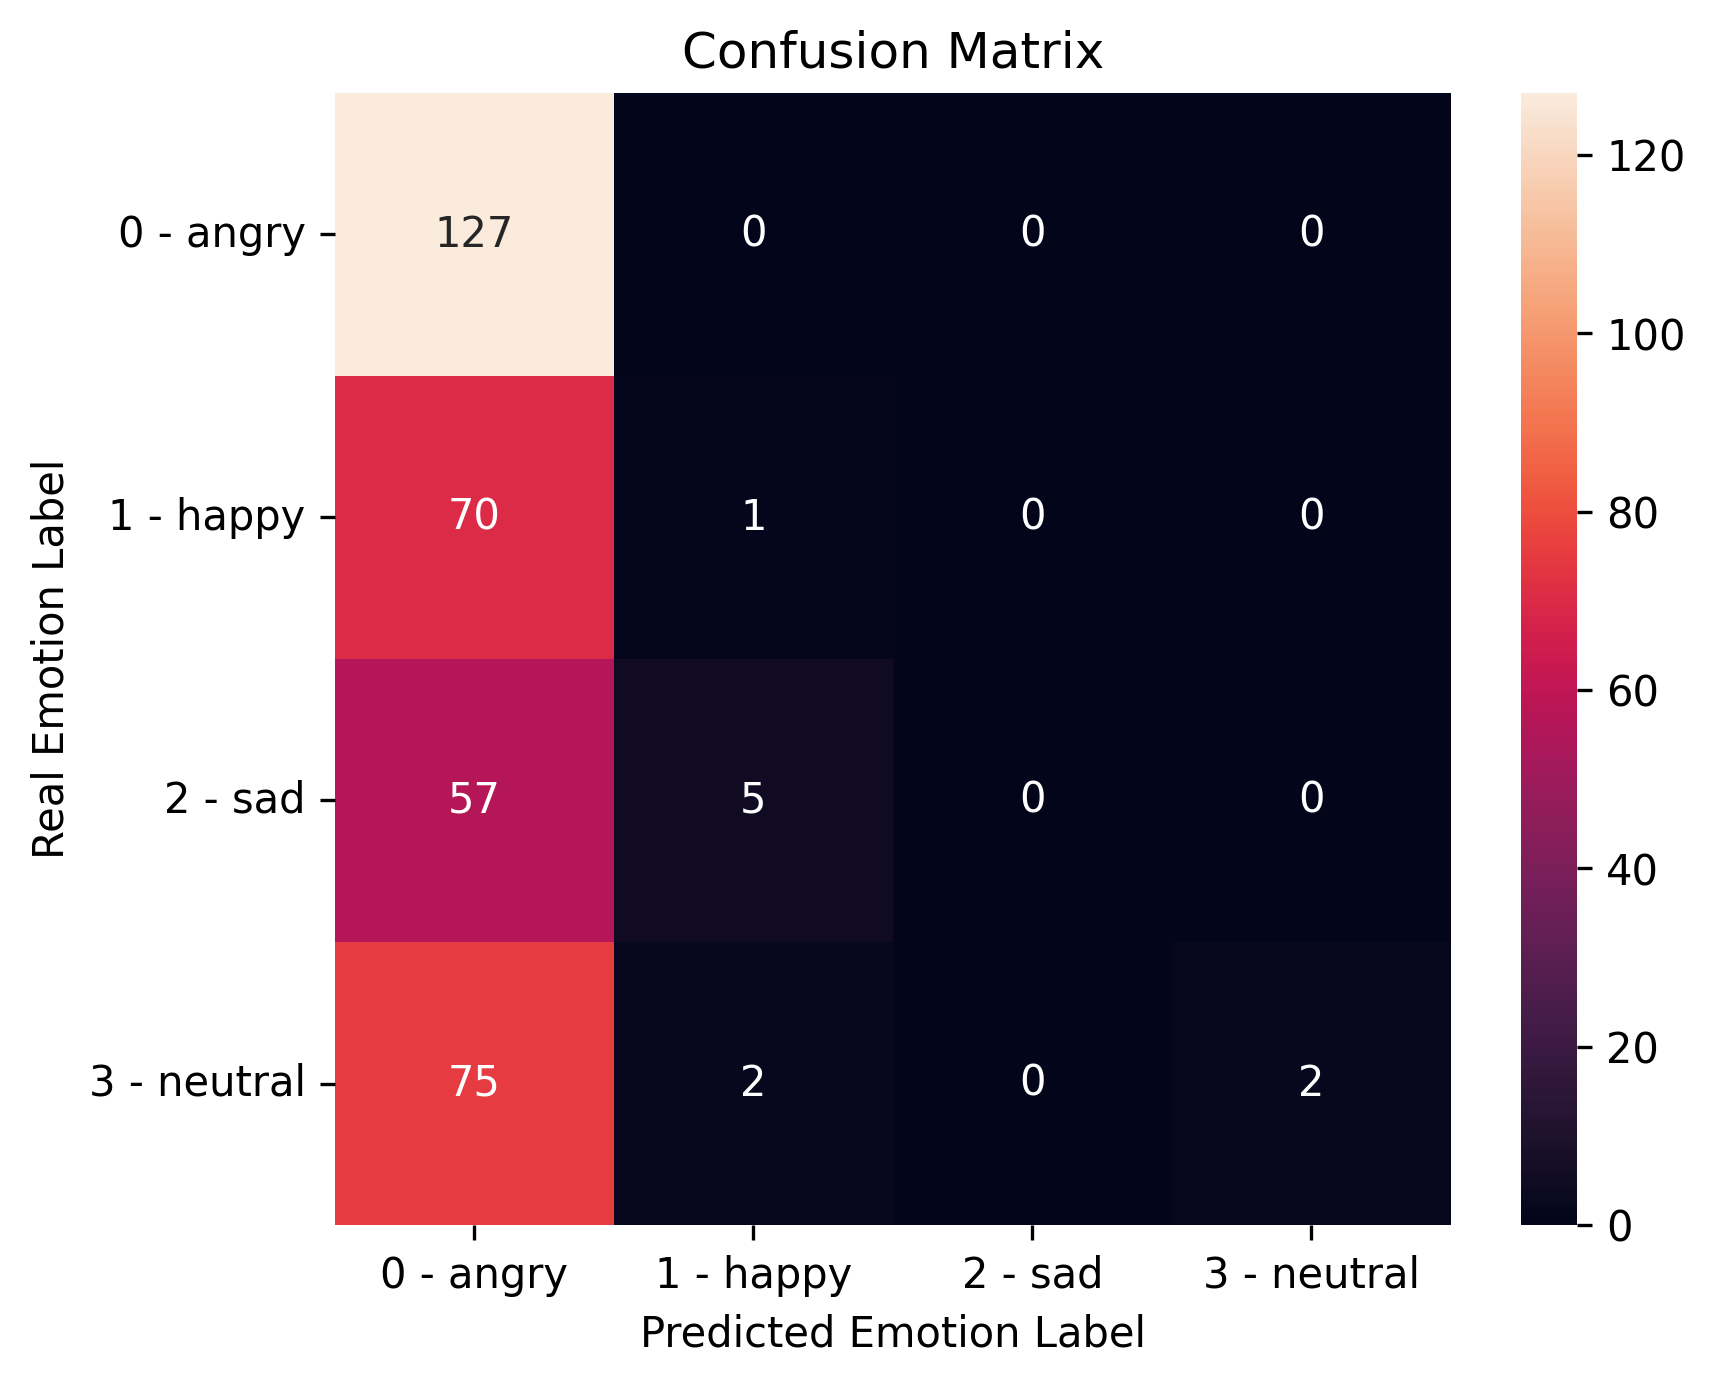
\includegraphics[width=\linewidth]{figs/4_5_discussion/emo_deep_cm.png}
		\caption{EMO-DB \ac{dl} model confusion matrix.}
	\end{subfigure}
	\newline
	\begin{subfigure}{.5\textwidth}
		\centering
		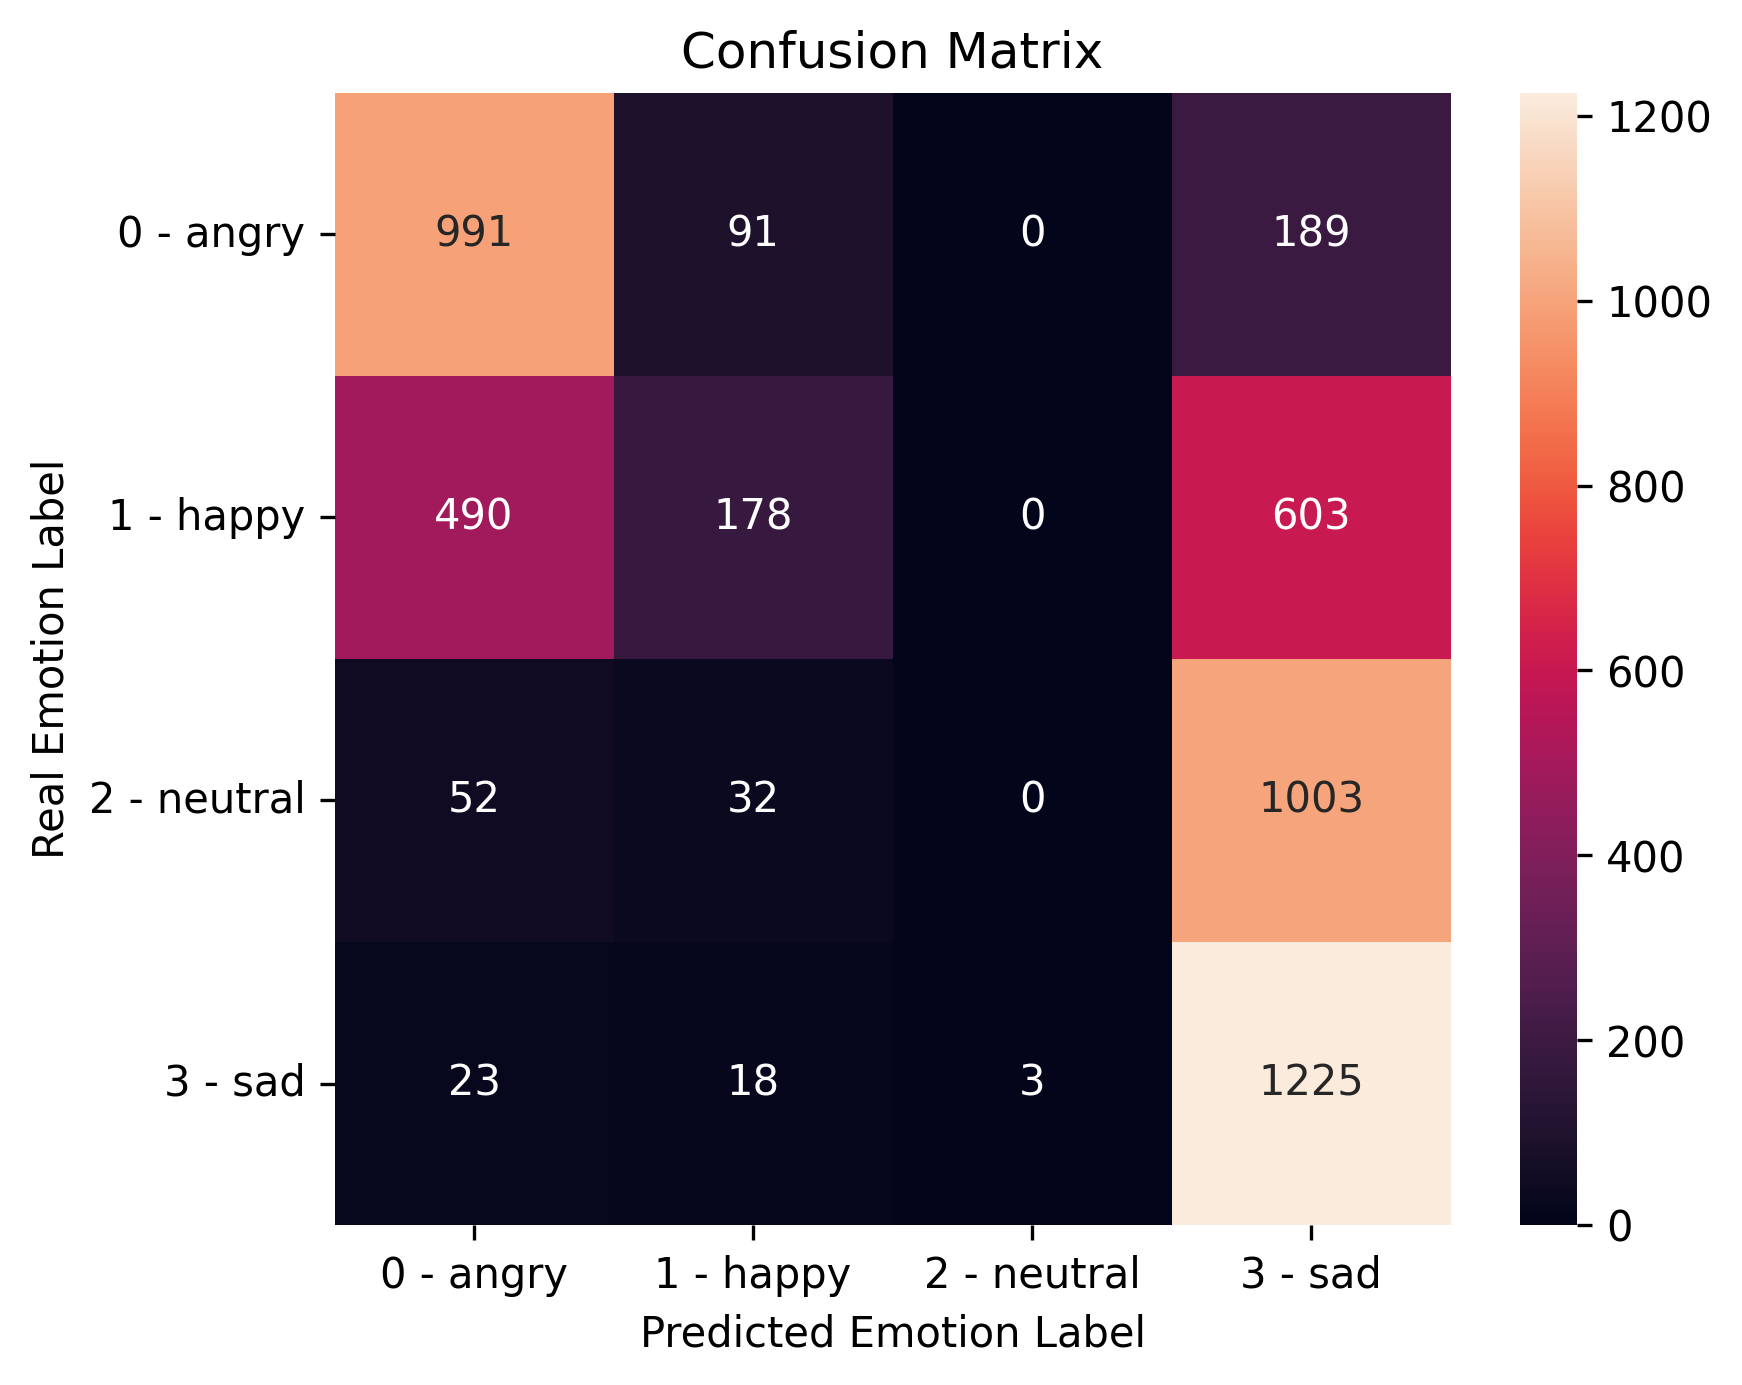
\includegraphics[width=\linewidth]{figs/4_5_discussion/cre_trad_cm.png}
		\caption{CREMA-D Traditional model confusion matrix.}
	\end{subfigure}%
	\begin{subfigure}{.5\textwidth}
		\centering
		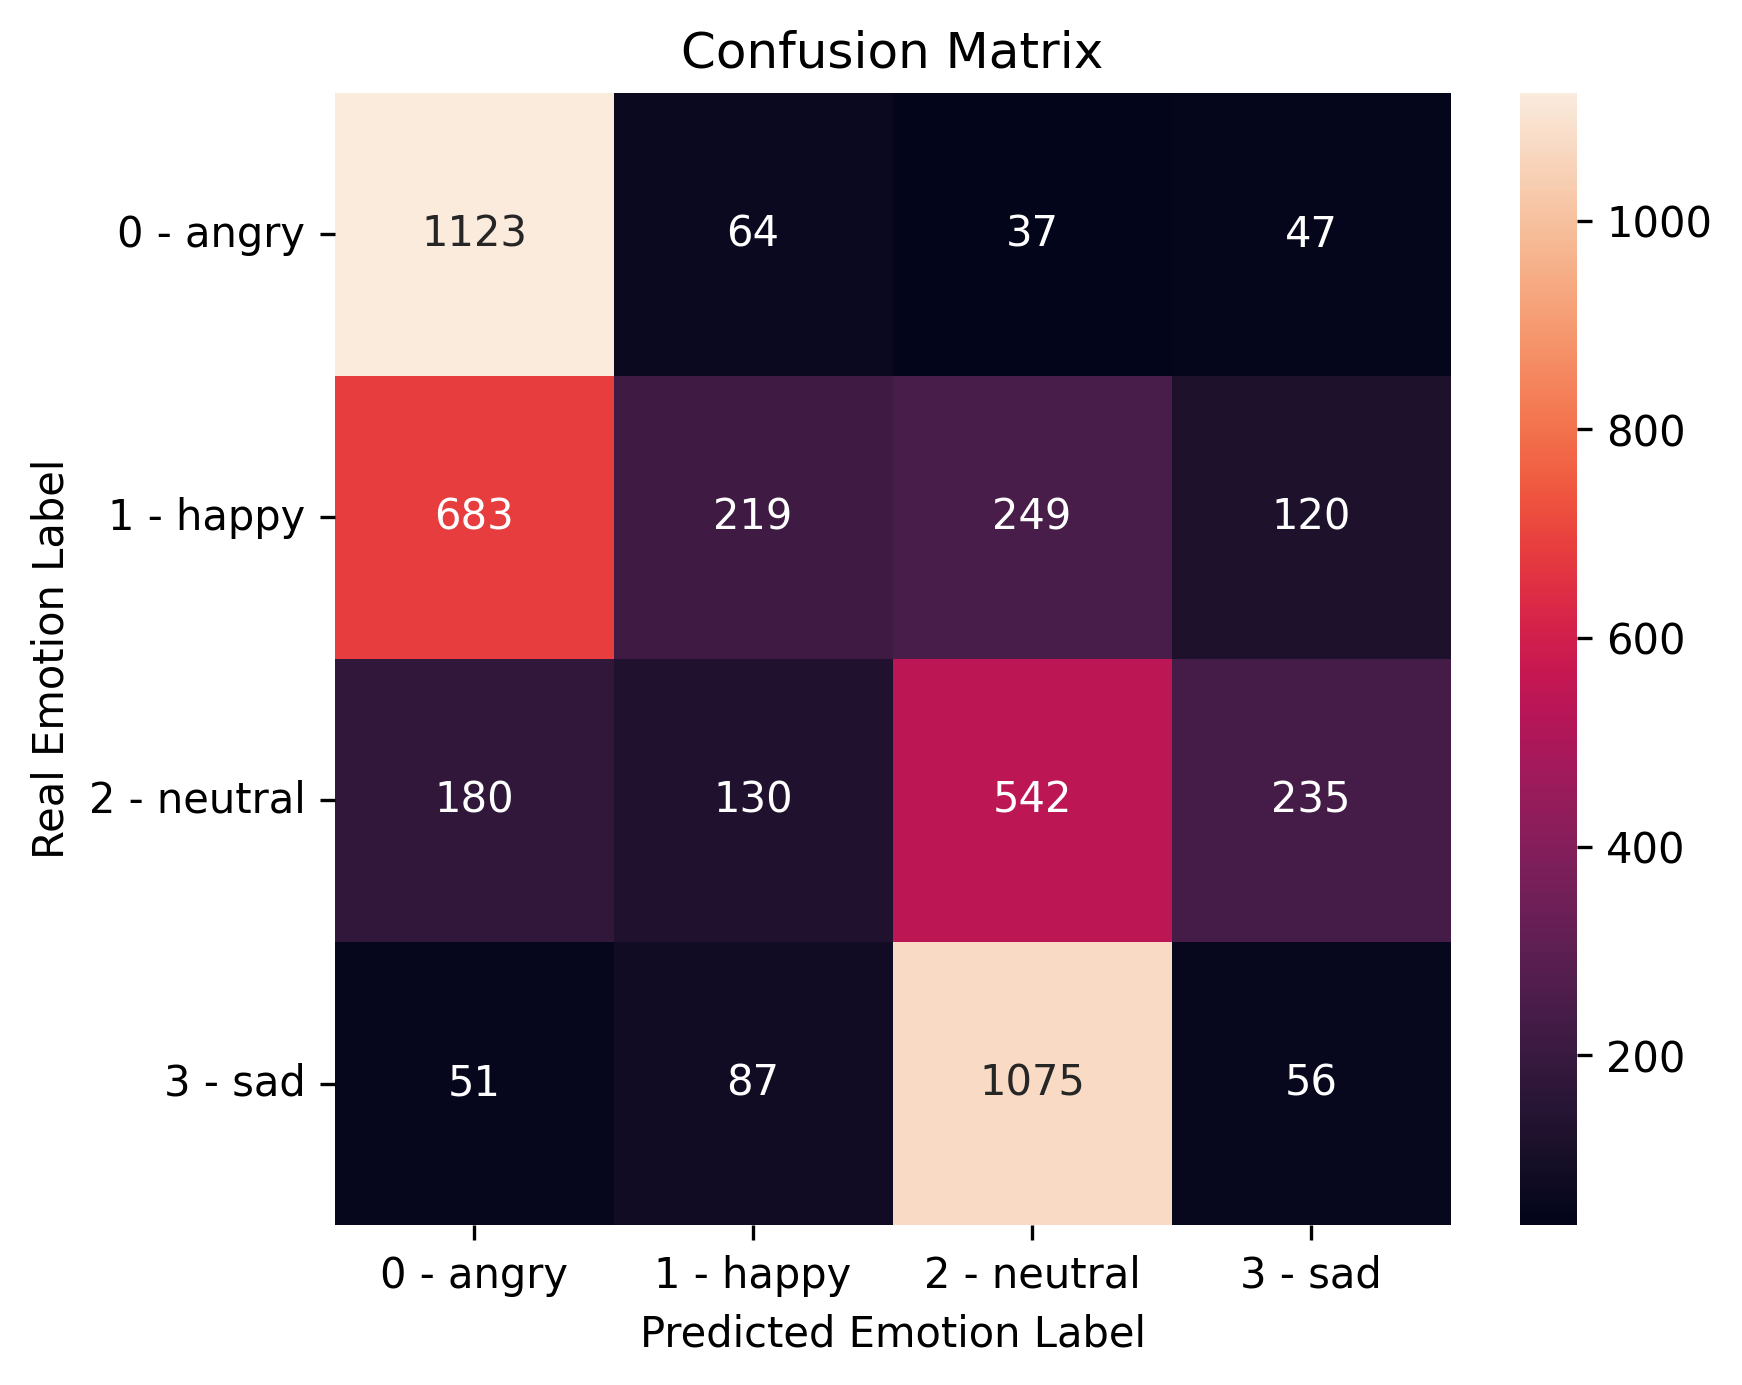
\includegraphics[width=\linewidth]{figs/4_5_discussion/cre_deep_cm.png}
		\caption{CREMA-D \ac{dl} model confusion matrix.}
	\end{subfigure}
	\caption{Final models confusion matrices on the eNTERFACE'05, EMO-DB and CREMA-D datasets.}
	\label{fig:final_cm}
\end{figure}


\paragraph{\ac{sota} Comparison}

The \ac{sota} results presented in Table \ref{tab:modelssoa} are not directly comparable, as authors use different data and evaluation methodologies. Additionally, some authors do not consider the emotion of excitement as happiness or perform different validation methods such as 10-fold \ac{cv}.

\begin{table}[H]
	\centering
	\caption{\ac{sota} classification models performance on \ac{iemo}.}
	\label{tab:modelssoa}
	\begin{tabular}{lccr}
		\toprule
		Model                      & Input & Evaluation Strategy & Accuracy (\%) \\
		\midrule
		\addlinespace[1mm]
		
		\multicolumn{4}{c}{Traditional Feature-Based Approaches} \\
		\midrule
		
		\begin{tabular}[l]{@{}l@{}}Ensemble of \ac{rf}, \ac{xgb}\\and Multilayer Perceptron\end{tabular} \cite{HandCraftedSahu} & \begin{tabular}[c]{@{}c@{}}8-dimensional audio\\features vector\end{tabular} & \begin{tabular}[c]{@{}c@{}}1 random 80:20\\train-test split\end{tabular} & 56.00 \\
		\addlinespace[1mm]
		
		\begin{tabular}[l]{@{}l@{}}Multi-level binary\\decision trees \cite{Lee2011}\end{tabular} & 384 audio features vector & 10 fold \ac{cv} & 58.46 \\
		\addlinespace[1mm]
		
		\rowcolor{LightCornflowerBlue}
		\ac{xgb} [Ours] & 33 audio features vector & 5-fold \ac{cv} & 60.69 \\
		\addlinespace[1mm]
		
		\ac{cnn} \cite{Issa2020}  & 193 audio features vector & 5-fold \ac{cv} & 64.30 \\
		\addlinespace[1mm]
		
		\midrule
		\addlinespace[1mm]
		\multicolumn{4}{c}{\acl{dl}-Based Approaches} \\
		\midrulecb
		
		\rowcolor{LightCornflowerBlue}
		Resnet50 [Ours] & 3-D Spectrogram Image & 5-fold \ac{cv} & 58.24 \\
		\addlinespace[1mm]
		
		\ac{cnn} and \ac{rnn} \cite{ma18b_interspeech} & Log-Spectrogram & 5-fold \ac{cv} & 64.22 \\
		\addlinespace[1mm]
		
		\begin{tabular}[l]{@{}l@{}}3-D attention-based\\convolutional \ac{rnn} \cite{8421023}\end{tabular} & Mel-Spectrogram & 10-fold \ac{cv} & 64.7 \\
		\addlinespace[1mm]
		
		\begin{tabular}[l]{@{}l@{}}\ac{cnn} and \ac{lstm}\\with attention \cite{Zhao2019}\end{tabular} & Mel-Spectrogram & 5-fold \ac{cv} & 67.0 \\
		\addlinespace[1mm]
		
		Quaternion \ac{cnn} \cite{Muppidi2021} & \begin{tabular}[c]{@{}c@{}}Mel spectrogram\\ encoded in an RGB\\quaternion domain\end{tabular} & 5-fold \ac{cv} & 70.46 \\
		\addlinespace[1mm]
		
		\bottomrule
	\end{tabular}
\end{table}
